\newif\ifpdf
\ifx\pdfoutput\undefined\relax
\else\ifnum\pdfoutput>0\relax
\pdftrue\fi\fi

\def\filedate{2002/01/07}
\def\docdate{2001/01/13}
\def\fileversion{1.203}
\def\basename{ntheorem}

\documentclass[11pt,oneside]{ltxdoc}

\usepackage{latexsym}
\usepackage[thmmarks,thref,noconfig]{ntheorem}
\usepackage[utf8x]{vietnam}
\usepackage{indentfirst}
\usepackage{ktv-buildnum}
\usepackage{hyperref}
\usepackage{url}
\usepackage{varioref}
\usepackage[varioref]{vnhook}
\usepackage{graphicx}

\newif\ifprint
%% taken from `pdpream.ble' generated from `powerdot.dtx'.
\usepackage{url}
\usepackage{xcolor}
\usepackage{enumitem}
\usepackage{pst-char}
\usepackage{listings}
\usepackage{array}
\usepackage{xkeyval}

\newbox\yaktmpbox

\newenvironment{thmbox}{%
	\setbox\yaktmpbox=\hbox\bgroup%
	\kern-\leftmargin
	\kern-6.45pt % value found by try-and-error. What is the exact one?
	\vbox\bgroup\ignorespaces%
}{%
	\egroup\egroup\fcolorbox{black}{yellow!20}{\box\yaktmpbox}%
}

\lstnewenvironment{command}{%
  \lstset{columns=flexible,frame=single,backgroundcolor=\ifprint\color{white}\else\color{blue!20}\fi,%
    xleftmargin=\fboxsep,xrightmargin=\fboxsep,escapeinside=`',gobble=1}\ttfamily}{}
\lstnewenvironment{example}[1][]{%
  \lstset{basicstyle=\footnotesize\ttfamily,columns=flexible,frame=single,%
    backgroundcolor=\ifprint\color{white}\else\color{yellow!20}\fi,xleftmargin=\fboxsep,%
    xrightmargin=\fboxsep,gobble=1,%
    }\lstset{#1}}{}
\def\option#1{%
	\ifprint
		\fcolorbox{black}{white}{\texttt{#1}}\vspace*{.2cm}%
	\else
		\fcolorbox{black}{red!20}{\texttt{#1}}\vspace*{.2cm}%
	\fi%
}
\def\exmacro#1{
	\ifprint
		\fcolorbox{black}{white}{\texttt{\bslash#1}}\vspace*{.2cm}%
	\else
		\fcolorbox{black}{blue!20}{\texttt{\bslash#1}}\vspace*{.2cm}%
	\fi%
}
\def\macro#1{
	\ifprint
		\fcolorbox{black}{white}{\texttt{\bslash#1}}\vspace*{.2cm}%
	\else
		\fcolorbox{black}{red!20}{\texttt{\bslash#1}}\vspace*{.2cm}%
	\fi%
}
\def\mktitledecor{%
  \rput[tl]{90}(-5.5,-25.51){%
    \psline[linewidth=1pt](0,1.5)(\paperheight,1.5)%
    \rput[lB](.075\paperheight,.5){\pscharpath[linecolor=blue!50,%
      fillcolor=yellow!20,fillstyle=solid,linewidth=.5pt]%
      {\Huge\bfseries\sffamily VietTUG, \url{http://viettug.org/}}%
    }%
    %\rput[rB](.925\paperheight,.5){\pscharpath[linecolor=blue!50,%
    %  fillcolor=yellow!20,fillstyle=solid,linewidth=.5pt]%
    %  {\Huge\bfseries Documentation}%
    %}%
    \psline[linewidth=1pt](0,0)(\paperheight,0)%
  }%
}
\makeatletter
\def\tableofcontents{\@starttoc{toc}}
\renewenvironment{theglossary}{%
  \section*{Version history}%
  \GlossaryParms \let\item\@idxitem \ignorespaces
}{}%
\def\DescribeMacros{\leavevmode\@bsphack
  \begingroup\MakePrivateLetters\Describe@Macros}
\def\Describe@Macros#1{\endgroup\strut
  \marginpar{\raggedleft
  \def\@tempa{#1}\count@\z@
  \XKV@for@o\@tempa\@tempa{%
    \ifnum\count@>\z@\\\fi\advance\count@\@ne
    \MacroFont\expandafter\string\@tempa
    \expandafter\SpecialUsageIndex\expandafter{\@tempa}%
  }}%
  \@esphack\ignorespaces
}
\def\DescribeOption#1{\leavevmode\@bsphack
              \marginpar{\raggedleft\PrintDescribeOption{#1}}%
              \SpecialOptionIndex{#1}\@esphack\ignorespaces}
\def\PrintDescribeOption#1{\MacroFont #1\ }
\def\SpecialOptionIndex#1{\@bsphack
    \index{#1\actualchar{\protect\ttfamily#1}
           (option)\encapchar usage}\@esphack}
\def\DescribeOptions#1{\leavevmode\@bsphack
  \marginpar{\raggedleft%\strut\emph{options}%
  \@for\@tempa:=#1\do{%
    \strut\MacroFont\@tempa\\\SpecialOptionIndex\@tempa
  }}\@esphack\ignorespaces}
\def\SpecialEnvIndex#1{\@bsphack
    \index{#1\actualchar{\protect\ttfamily#1}
           (environment)\encapchar usage}\@esphack}
\def\changes@#1#2#3{%
  \protected@edef\@tempa{%
    \noexpand\glossary{\textbf{#1}\hfill\emph{(#2)}%
    \levelchar
    \ifx\saved@macroname\@empty
      \space\actualchar\generalname
    \else
      \expandafter\@gobble\saved@macroname
      \actualchar\string\verb\quotechar*%
      \verbatimchar\saved@macroname\verbatimchar
    \fi
    :\levelchar #3}%
  }%
  \@tempa\endgroup\@esphack
}
\makeatother
\def\PrintChangesX{%
  \begingroup
    \let\efill\relax
    \PrintChanges
  \endgroup
}
\def\PrintIndexX{%
  \begingroup
    \setcounter{IndexColumns}{2}
    \setlength{\columnsep}{18pt}%
    \setlength{\columnseprule}{.4pt}%
    \PrintIndex
  \endgroup
}
\def\larg#1{{\ttfamily\char`\<}\meta{#1}{\ttfamily\char`\>}}
\let\pf\textsf
\newcolumntype{d}{c|l}
\newcolumntype{e}{c|c|c|c}
\RecordChanges
\CodelineIndex
\newcounter{FAQ}
\def\question{%
  \stepcounter{FAQ}%
  \parskip4pt plus 2pt minus 1pt
  \itemsep4pt plus 2pt minus 1pt
  \parsep4pt plus 2pt minus 1pt
  \item[\textbf{Q\arabic{FAQ}}]%
}
\def\answer{%
  \parskip0pt
  \itemsep0pt
  \parsep0pt
  \item[\ding{42}]%[\textbf{A\arabic{FAQ}}]%
}
\endinput
%%
%% End of file `pdpream.ble'.


\parindent0pt
%\hfuzz2pt
\setlength{\textwidth}{360pt}

\setlength{\hoffset}{1cm}
\setlength{\voffset}{-1cm}
\setlength{\textwidth}{13.5cm}
\setlength{\textheight}{23cm}

\MakeShortVerb{\|}
\def\envfont{\normalfont\ttfamily}
\def\deflabel#1{\ttfamily #1\hfill}
\def\deflist#1{\begin{list}{}{\settowidth\labelwidth{\ttfamily #1}%
                              \setlength\leftmargin\labelwidth
                              \addtolength\leftmargin\labelsep
                              \let\makelabel\deflabel}}
\def\enddeflist{\end{list}}

\def\packedlist#1{%
   \begin{list}{}{\settowidth\labelwidth{#1}\setlength\leftmargin\labelwidth
                  \addtolength\leftmargin\labelsep
                  \topsep=0pt\itemsep=0.05cm\parsep=0.05cm
                  \let\makelabel\nlabel}}
\def\endpackedlist{\end{list}}
\makeatletter
\def\packeddescr{%
   \begin{list}{}{\leftmargin0.5cm
                  \labelwidth\z@\itemindent-\leftmargin
                  \topsep=0pt\itemsep=0.05cm\parsep=0.05cm
                  \let\makelabel\nlabel}}
\def\endpackeddescr{\end{list}}

\def\Codelabel#1{\@bsphack  
 \protected@write\@auxout{}{\string\newlabel{#1}{{\number\the
           \c@CodelineNo}{\thepage}}}\@esphack}
\newcounter{tmpcount}
\def\Coderef#1#2{\setcounter{tmpcount}{0}\@ifundefined{r@#1}\relax
          {\setcounter{tmpcount}{\ref{#1}}}\relax
          \addtocounter{tmpcount}{#2}\arabic{tmpcount}}
\makeatother

\def\nlabel#1{#1\hfill}
\def\nlist#1{\begin{list}{}{\settowidth\labelwidth{#1}%
                            \setlength\leftmargin\labelwidth
                            \addtolength\leftmargin\labelsep
                            \let\makelabel\nlabel}}
\def\endnlist{\end{list}}
\def\DANGER{{\LARGE\textbf{! }\rule{0pt}{2ex}}}
\def\env{\meta{env}}
\def\envx{\meta{env'}}

\theoremstyle{marginbreak}
\theoremheaderfont{\normalfont\bfseries}\theorembodyfont{\slshape}
\theoremsymbol{\ensuremath{\diamondsuit}}
\theoremseparator{:}
\newtheorem{Theorem}{Theorem}

\theoremstyle{changebreak}
\theoremsymbol{\ensuremath{\heartsuit}}
\theoremindent0.5cm
\theoremnumbering{greek}
\newtheorem{Lemma}{Lemma}

\theoremindent0cm
\theoremsymbol{\ensuremath{\spadesuit}}
\theoremnumbering{arabic}
\newtheorem{Corollary}[Theorem]{Corollary}

\theoremstyle{change}
\theorembodyfont{\upshape}
\theoremsymbol{\ensuremath{\ast}}
\theoremseparator{}
\newtheorem{Example}{Example}

\theoremstyle{plain}
\theoremsymbol{\ensuremath{\clubsuit}}
\theoremseparator{.}
\newtheorem{Definition}{Definition}

\theoremheaderfont{\sc}\theorembodyfont{\upshape}
\theoremstyle{nonumberplain}
\theoremseparator{}
\theoremsymbol{\rule{1ex}{1ex}}
\newtheorem{Proof}{Proof}%


\begin{document}

% =====================================================================

\title{%An Extension of the \LaTeX-Theorem Evironment%
	%\thanks{This 
	%         file has version number \fileversion{}, last revised \filedate.}
	Mở rộng môi trường định lý của \LaTeX{}
}
\author{%
	Wolfgang May\thanks{\url{may@informatik.uni-freiburg.de}}
	\qquad 
	Andreas Schlechte\thanks{\url{ntheorem@andreas-schlechte.de}}\\[2mm]
	\emph{\underline{Biên dịch:}} kyanh\thanks{\url{kyanh@o2.pl}}%
}
\date{%
	Bản dịch số \textbf{\the\buildnum}\\[2mm]
	\fcolorbox{black}{red!20}{cho \textbf{ntheorem} bản \textbf{1.24} (2004/09/20)}}

\maketitle          

% =====================================================================

\begin{abstract}
%\noindent
%%  |ntheorem.sty| is a package for handling theorem-like environments.
%%  Aditionally to several features for defining the layout of
%%  theorem-like environments which can be regarded to be standard
%%  requirements for a theorem-package, it provides solutions for
%%  two related problems: placement of endmarks and generation of
%%  lists of theorem-like environments.
|ntherem.sty| là gói thể hiện các môi trường (tựa) định lý.
Bên cạnh các tính năng giúp thay đổi cách thể hiện môi trường (tựa) định lý,
gói còn giúp giải quyết vài vấn đề liên quan: đặt dấu kết thúc (|endmarks|),
tạo bảng liệt kê các định lý.

%%  In contrast to former approaches, it solves the problem of 
%%  setting endmarks of theorem-like environments (theorems, 
%%  definitions, examples, and proofs) \emph{automatically} at the 
%%  right positions, even if the environment ends with a |displaymath| 
%%  or (even nested) list environments, it also copes with the 
%%  |amsmath| package.
%%  This is done in the same manner as the handling of labels by
%%  using the |.aux| file.
\medskip
Trái với các cách tiếp cận trước đây, gói giải quyết vấn đề đặt dấu
kết thúc (|endmarks|) cho các môi trường tựa định lý (|theorem|,
|definition|, |example|, |proof|) một cách tự động, chính xác, ngay cả
đối với môi trường kết thúc bởi môi trường |displaymath| hoặc môi trường
danh sách (thậm chí các môi trường này có thể lồng nhau -- |nested|);
nhờ đó giải quyết được hoàn toàn các trục trặc khi dùng gói |amsmath|.
Nguyên lý làm việc của gói giống như cách \LaTeX{} điều khiển việc
đặt nhãn, bằng cách sử dụng các tập tin |.aux|.

%%  It also introduces the generation of lists of theorem-like 
%%  environments in the same manner as |listoffigures|. Additionally,
%%  more comfortable referencing is supported.
\medskip
Gói cung cấp lệnh để tạo danh sách các môi trường tựa định lý,
tương tự như khi liệt kê các hình vẽ bằng |\listoffigures|.
% Ngoài ra, gói hỗ trợ 

%%  After running \LaTeX\ several times (depending on the complexity
%%  of references, in general, three runs are sufficient), the endmarks 
%%  are set correctly, and theoremlists are generated.
\medskip
Sau khi biên dịch tài liệu vài lần (số lần tuỳ thuộc vào sự phức tạp
của các tham khảo chéo; thường thì ba lần là đủ), các dấu kết thúc (|endmarks|)
sẽ được đặt đúng chỗ, và danh sách các định lý sẽ được tạo ra.

%%  Since |ntheorem.sty| uses the standard \LaTeX\ |\newtheorem|
%%  command, existing documents can be switched to
%%  |ntheorem.sty| without having to change the |.tex| file.
%%  Also, it is compatible with \LaTeX\ files using |theorem.sty| 
%%  written by Frank Mittelbach.
\medskip
Do gói |ntheorem.sty| sử dụng lệnh |\newtheorem| của \LaTeX{} chuẩn,
các tài liệu cũ có thể chuyển qua dùng gói mà không cần thay đổi nội
dung. Ngoài ra, gói còn tương thích với các tài liệu dùng gói |theorem.sty|
của Frank Mitterbach.
\end{abstract}

\newpage

\tableofcontents

\pagebreak

% =====================================================================

\section{Giới thiệu. Ghi chú}

%% For our purposes here, ``theorems'' are labelled enunciations,
%% often set off from the main text by extra space and a font change.
%% Theorems, corollaries, conjectures, definitions, examples, 
%% remarks, and proofs are all instances of ``theorems''.  
%% The ``header'' of 
%% these structures is composed of the type of the structure 
%% (such as \textsc{Theorem} or \textsc{Remark}), a number 
%% which serializes the instances of the same type throughout the
%% document, and an optional name (such as ``Correctness Theorem'').
Một môi trường tựa định lý, ta gọi tắt là |THM|, được minh họa
như ở Hình~\ref{fig:THM}. Với mỗi |THM|, các tên |định lý|, |hệ quả|, |bổ đề|, |tiên đề|,
|định nghĩa|, |ví dụ|, |ghi chú|, |chứng minh|,\ldots
được gọi là \emph{tên của} |THM|.
Phần |header| của |THM| bao gồm tên của |THM|, chỉ số của |THM|,
tên tuỳ chọn (hay tên riêng) của |THM|. Phần nội dung của |THM|
còn gọi là \emph{thân} của |THM|. Để ý rằng, tên của |THM| khác
với tên của môi trường |THM|.\footnote{Trong thực tế, thường tên
của môi trường \texttt{THM} và tên của \texttt{THM} có sự tương ứng
1-1, ví dụ \texttt{menhde} ứng với \texttt{Mệnh đề},
\texttt{dinhly} ứng với \texttt{Định lý}. Do đó, trong đa số trường hợp,
sự phân biệt này không có ý nghĩa quan trọng\ldots --- kyanh}
Trong ví dụ sau,
\begin{example}
  \newtheorem{foobar}{Menh de}
\end{example}
ta có |THM| với tên là |Menh de|, nhưng tên của môi trường
tương ứng là |foobar|. Đôi khi, ta sẽ gọi \emph{môi trường} |THM| thay cho
\emph{tên của môi trường} |THM|.
%% dùng để chỉ loại của cấu trúc (ví dụ định lý hay
%% định nghĩa), chỉ số của cấu trúc và tên tuỳ chọn (ví dụ |Tiên đề chọn|).
%% Các (tựa) định lý thường phải được trình bày rõ ràng, tách biệt
%% với các phần khác cùa tài liệu, bằng cách thêm các khoảng trắng
%% thích hợp, thay đổi kiểu chữ. 

%% The layout of theorems can be changed by parameters as the fonts
%% of the header and the body, the way how to arrange the headers,
%% the indentation, and the way of numbering it.
%% Confronted with these requirements, |theorem.sty|, a style for 
%% dealing with theorem layout was developed by Frank Mittelbach
%% which was the standard theorem-environment for long time.
\medskip
Cách thể hiện |THM| có thể được thay đổi nhờ các tham số về
kiểu chữ cho |header|, cho thân |THM|, các bố trí |header|, khoảng trắng
thụt đầu dòng, cách đánh số,\ldots Để thỏa mãn các yêu cầu thay đổi này,
gói |theorem.sty| của Fran Mittelbach đã được viết và trở thành
gói chuẩn của \LaTeX{} từ rất lâu.

%% But then the desire for additional features like ``endmarks''
%% and ``theorem-lists'' arose. 
%% Two extensions of |theorem.sty| were developped: One for handling 
%% endmarks, |thmmarks.sty| and one for generating lists, |newthm.sty|. 
%% Thus, Frank Mittelbach suggested to combine the new features into 
%% one ``standard-to-be'' package. 
%% And now, here it is.
\medskip
Tuy nhiên, các tính năng khác nhưng dấu kết thúc |endmarks|, danh sách
các |theorem| vẫn chưa được hỗ trợ bởi gói chuẩn đó. Giải quyết vấn đề này,
có hai mở rộng của gói |theorem.sty| được phát triển: một gói chuyên về
điều khiển |endmarks|, gói |thmmarks.sty|, và một gói chuyên về liệt
kê danh sách |THM|, gói |newthm.sty|. Sau đó, Frank Mittelbach đề nghị
kết hợp các hỗ trợ của hai gói này vào cùng một gói mới (sẽ là chuẩn).
Đó chính là gói |ntheorem.sty| ;)

\begin{figure}[bht]
\begin{center}
	\ifpdf
		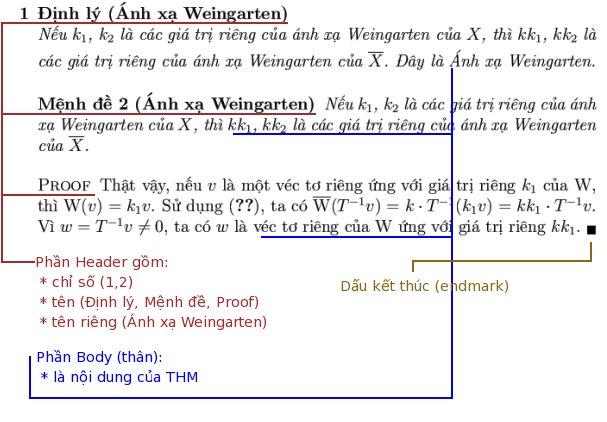
\includegraphics[scale=.6]{thm.png}
	\else
		\includegraphics[scale=.6]{thm.ps}
	\fi
\end{center}
\caption{Môi trường THM}
\label{fig:THM}
\end{figure}

% =====================================================================

%\section{The User-Interface}
\section{Sử dụng gói}

% =====================================================================

%\subsection{How to include the package}
\subsection{Nạp gói}

%The package |ntheorem.sty| is included by
Gói |ntheorem.sty| có thể nạp như sau
\begin{command}
  \usepackage[`\meta{options}']{ntheorem}
\end{command}
%% where the optional parameter \meta{options} selects predefined
%% configurations and special requirements. 
với \meta{options} là danh sách các tuỳ chọn và các yêu cầu đặc biệt.

%% The following \meta{options} are available by now, concerning three
%% independent issues:
\medskip
Các tuỳ chọn được cho nhờ \meta{options} như sau: % liên quan đến ba vấn đề độc lập:
\begin{description}
%% \item[Predefining environments:] (see Section~\ref{sec:standard})
%%   With [standard] and [noconfig], it can be chosen, if and what
%%   file is used for activating a (user-defined) standard set of 
%%   theorem environments.
\item\DescribeOptions{standard,noconfig}\option{standard} \option{noconfig}\\
	xem Mục~\vref{sec:standard}. Với một
	trong hai tùy chọn |standard| và |noconfig|,
	bạn có thể lựa chọn việc sử dụng hoặc không tập hợp
	các môi trường |THM| đã được định nghĩa sẵn.
%% \item[Compatibility with amsthm:] option [amsthm] provides 
%%        compatibility with the theorem-layout
%%       commands of the |amsthm|-package (see Section~\ref{sec:amslatex}).
\item\DescribeOption{amsthm}\option{amsthm}\\
	tùy chọn |amsthm| khi được dùng sẽ bảo đảm tính tương thích với các môi trường
	|THM| cung cấp bởi gói |amsthm|. Xem Mục~\vref{sec:amslatex}.
%\item[Activation of endmarks:]
\item\DescribeOption{thmmarks}\option{thmmarks}\\
%% [thmmarks] enables the automatical placement of endmarks 
%%     (see \ref{sec:general}); when using the |amsmath|-package,
%%     [thmmarks] must be complemented by [amsmath] 
%%     (see Section~\ref{sec:amslatex}).
	tuỳ chọn |thmmarks| đồng ý để gói |ntheorem.sty| tự động đặt dấu kết thúc
	(|endmarks|) (xem Mục~\ref{sec:general}); khi dùng với gói |amsthm|,
	tùy chọn |thmmarks| phải được dùng kèm với tuỳ chọn |amsmath|.
	Xem thêm ở Mục~\ref{sec:amslatex}.
%% \item[Activation of extended reference features:]
%% [thref] enables the extended reference features 
%%     (see Section~\ref{sec-ExtRef}); when using the |amsmath|-package,
%%     [thref] must be complemented by [amsmath] 
%%     (see Section~\ref{sec:amslatex}).
\item\DescribeOption{thref}\option{thmref}\\
	tuỳ chọn |thref| cho phép mở rộng khả năng tham khảo chéo. Xem Mục~\vref{sec-ExtRef};
	khi dùng với gói |amsthm|, tuỳ chọn này phải đi kèm với tuỳ chọn |amsmath|.
	Xem thêm ở Mục~\ref{sec:amslatex}.
%% \item[Compatibility with hyperref:] option [hyperref] provides
%%       compability with the |hyperref|-package 
%%       (see section~\ref{sec:hyperref}).
\item\DescribeOption{hyperref}\option{hyperref}\\
	tuỳ chọn |hyperref| bảo đảm tương thích với gói |hyperref|.
	Xem Mục~\vref{sec:hyperref}.
\end{description}

Dưới đây là một ví dụ:
\begin{example}
  \usepackage{hyperref}
  \usepackage[hyperref,thmmarks,noconfig]{ntheorem}
\end{example}
Với cách nạp gói như trên, bạn sẽ phải tự định nghĩa các môi trường |THM|,
các dấu kết thúc sẽ được định vị tự động. Vì ta dùng gói |hyperref|,
ta phải bảo đảm tính tương thích nhờ tuỳ chọn |hyperref|.

% =====================================================================

%\subsection{Defining New Theorem Sets}
\subsection{Định nghĩa THM mới}

\DescribeMacro{\newtheorem}\macro{newtheorem}\\
%% The syntax and semantics is exactly the same as in standard
%% \LaTeX{}: the command |\newtheorem| defines a new ``theorem set'' 
%% or ``theorem-like structure''.
%% Two required arguments name the new environment set and give the 
%% text to be typeset with each instance of the new ``set'', while
%% an optional argument determines how the ``set'' is enumerated:
Cú pháp của lệnh hoàn toàn giống như của lệnh chuẩn |\newtheorem|.
Lệnh sẽ định nghĩa một |THM| mới. Có hai tham số bắt buộc là tên
của môi trường và tên của |THM|. Tham số bổ sung chỉ ra cách đánh số
môi trường.
\begin{description}
   \item\exmacro{newtheorem\{vidu\}\{Ví dụ\}}\\
%%       The theorem set {\envfont foo} (whose name is \texttt{bar})
%%       uses its own counter.
	Định nghĩa môi trường |vidu|, với tên là |Ví dụ|
	(như vậy, bạn sẽ có |Ví dụ 1|, |Ví dụ 2|, \ldots). Môi trường
	này sử dụng bộ đếm riêng |vidu|, và bạn có thể thay đổi giá trị
	giá trị bộ đếm này, chẳng hạn |\setcounter{vidu}0|.
   \item\exmacro{newtheorem\{vidu2\}{[vidu]}\{Ví dụ khác\}}\\
%%       The theorem set {\envfont foo2} (printed name \texttt{bar2})
%%       uses the same counter as the theorem set \texttt{foo}.
	Định nghĩa môi trường |vidu2|, với tên là |Ví dụ khác|.
	Môi trường này sẽ sử dụng cùng bộ đếm của môi trường |vidu|
	trong ví dụ trước.
   \item\exmacro{newtheorem\{baitap\}\{Bài tập\}{[section]}}\\
%%       The theorem set {\envfont foo3} (printed name \texttt{bar}) is
%%       enumerated within the counter \texttt{section}, i.e.\ with every
%%       new |\section| the enumeration begins again with 1, and
%%       the enumeration is composed from the section-number and the
%%       theorem counter itself.
	Định nghĩa môi trường |baitap| (với tên là |Bài tập|), sử
	dụng bộ đếm thay đổi theo mục (|section|). Nếu bạn đang ở Mục số 5 chẳng hạn,
	bạn sẽ có |Bài tập 5.1|, |Bài tập 5.2|, \ldots Mỗi khi chuyển qua mục mới,
	bộ đếm sẽ được đặt về không, nghĩa là bạn sẽ có |Bài tập 6.1|, |Bài tập 6.2|, \ldots,
	|Bài tập 7.1|, |Bài tập 7.2|, \ldots
\end{description}

%% For every environment \meta{name}\ defined by |\newtheorem|,
%% \emph{two} enviroments \meta{name} and \meta{name|*|}\ are defined.
%% In the main document, they have exactly the same effect, but
%% the latter causes no entry in the respective list of theorems
%% (cf.\ |\section| and |\section*|), see also Section 
Khi gọi lệnh |\newtheorem| để tạo môi trường \meta{name}, thực ra sẽ có hai môi
trường được tạo ra, là \meta{name} và \meta{name|*|}. Điểm khác biệt duy nhất
giữa hai môi trường  này, cũng giống như sự khác biệt duy nhất giữa hai lệnh
|\section| và |\section*|, là môi trường \meta{name|*|} sẽ không đưa |THM|
vào trong danh sách liệt kê các |THM|. Trong các ví dụ ở trên, bạn sẽ có chẳng hạn
hai môi trường |baitap| và |baitap*|. Xem thêm Mục~\vref{sec:thmlists}.

\medskip
\DescribeMacro\renewtheorem\macro{renewtheorem}\\
%%
%% Theorem sets can be redefined by |\renewtheorem|, with the same arguments
%% as explained for |\newtheorem|. When redefining a theorem set, the 
%% counter is not re-initialized. 
Định nghĩa lại môi trường đã có. Cách dùng tương tự như của |\newtheorem|.
Bộ đếm sẽ được khởi tạo lại.

% =====================================================================

%% \subsection{Defining the Layout of Theorem Sets}
\subsection{Thay đổi kiểu dáng}

\label{sec:general}

%% For theorem-like environments, the user can set parameters
%% by setting several switches and then calling |\newtheorem|.
%% The layout of a theorem set is defined with the values of the switches
%% at the time |\newtheorem| is called.
Với các môi trường tựa định lý, bạn có thể thay đổi vài tham số (tuỳ chọn) trước
khi gọi lệnh |\newtheorem| để tinh chỉnh cách thể hiện môi trường
như ý bạn; các cài đặt nhờ tham số đó sẽ có tác dụng mỗi khi bạn
sử dụng môi trường.

% =====================================================================

%% \subsubsection{Common Parameters for all Theorem Sets}
\subsubsection{Các tham số chung}

\DescribeMacro\theorempreskipamount
\DescribeMacro\theorempostskipamount
\macro{theorempreskipamount} \macro{theorempreskipamount}\\ 
%% These additional parameters affect the vertical space around 
%% theorem environments:
%% |\theorempreskipamount| and |\theorempostskipamount| define,
%% respectively, the spacing before and after such an environment.
%% These parameters apply for all theorem sets and can be manipulated
%% with the ordinary length macros.  They are rubber lengths,
%% (`\textsf{skips}'), and therefore can contain \texttt{plus} and
%% \texttt{minus} parts.
Các tham số bổ sung này ảnh hưởng đến khoảng cách theo chiều đứng --
trên (|\theorempreskipamount|) và dưới (|\theorempostskipamount|) môi trường |THM|.
Hai tham số này ảnh hưởng đến mọi môi trường |THM| và có thể điều chỉnh
nhờ các lệnh thông thường điều khiển biến độ dài. Chúng là các chiều dài
dạng |rubber|, vì thế có thể chứa các phần với dấu cộng hoặc trừ.

%\subsubsection{Parameters for Individual Sets}
\subsubsection{Cho từng THM cụ thể}

%% The layout of individual theorem sets can be further determined
%% by switches controlling the appearance of the headers and the
%% header-body-layout:
Cách thể hiện của mỗi |THM| có thể tinh chỉnh nhờ các lệnh điều khiển sau đây.

\begin{description}
\item
\DescribeMacro\theoremstyle
  \exmacro{theoremstyle\{\meta{style}\}}\\
%%  The general structure of the 
%%  theorem layout is defined via its |\theoremstyle|. |\ntheorem|
%%  provides several predefined styles including those of
%%  Frank Mittelbach's |theorem.sty| 
	Xác định kiểu dáng của |THM|. Các kiểu được cung cấp với với |\ntheorem|
	bao gồm cả kiểu có trong gói |theorem.sty|. Xem liệt kê các kiểu
	ở Mục~\vref{sec:predefdstyles}.
%  Additional styles can be defined by |\newtheoremstyle| 
	Ở Mục~\vref{sec:newtheoremstyle} có nói về cách định nghĩa kiểu mới.
\item
\DescribeMacro\theoremheaderfont
  \exmacro{theoremheaderfont\{\meta{fontcmds}\}}\\
  %% The theorem header is set
  %%in the font specified by \meta{fontcmds}.
  Dùng \meta{fontcmds} để xác định |font| cho phần |header| của |THM|

%%   In contrast to |theorem.sty|, |\theoremheaderfont| can be set 
%%   individually for each environment type. 
	Không như |theorem.sty|, lệnh |\theoremheaderfont| cho phép đổi
	|font| cho từng kiểu |THM|.
\item
\DescribeMacro\theorembodyfont
  \exmacro{theorembodyfont\{\meta{fontcmds}\}}\\
  %The theorem body is set
  %%in the font specified by \meta{fontcmds}.
  Xác định |font| cho phần thân (nội dung) |THM|.
\item 
\DescribeMacro\theoremseparator
  \exmacro{theoremseparator\{\meta{sep}\}}\\
%%\meta{thing} %%separates the 
%%   header from the body of the theorem-environment. 
%%   E.g., \meta{thing} can be
%%   ``:'' or ``.''.
	Dùng \meta{sep} để ngăn cách phần |header| và phần thân của |THM|.
	Thường thì \meta{sep} là dấu hai chấm (|:|) hoặc chấm (|.|).
\item 
\DescribeMacro\theoremindent
%%   |\theoremindent{|\meta{dimen}|}| can be used to indent the theorem wrt.\
%%   the surrounding text.
	\exmacro{theoremindent\{\meta{dimen}\}}\\
	dùng để xác định |indent| (khoảng cách so với lề bên trái).

\DANGER
%% It's a `\textsf(dimen)', so the user shouldn't try to specify a
%% \texttt{plus} or \texttt{minus} part, cause this leads to an error.
	Ở đây, \meta{dimen} là kích thước thật sự. Nếu bạn dùng kiểu |rubber|
	với các dấu |plus| hoặc |minus| trong phần \meta{dimen}, bạn sẽ gặp lỗi.
\item
\DescribeMacro\theoremnumbering
  \exmacro{theoremnumbering\{\meta{style}\}}\\
%%   specifies the appearance of
%%   the numbering of the theorem set. Possible \meta{styles} are
   Kiểu đánh số cho |THM|. Các giá trị có thể là:
  |arabic| (default), |alph|, |Alph|, |roman|,
  |Roman|, |greek|, |Greek| và |fnsymbol|. 

%%   Clearly, if a theorem-environment uses the counter of another
%%   environment type, also the numbering style of that environment
%%   is used. 
	Rõ ràng, nếu môi trường |THM| sử dụng bộ đếm từ môi trường |XYZ| khác,
	thì kiểu đánh số của môi trường |THM| sẽ thừa hưởng từ |XYZ|.
\item
\DescribeMacro\theoremsymbol
  \exmacro{theoremsymbol\{\meta{thing}\}}\\
%%   This is only active if
%%   |ntheorem.sty| is loaded with option |[thmmarks]|. 
%%   \meta{thing} is set as an endmark at the end of every instance
%%   of the environment.
%%   If no symbol should appear, say |\theoremsymbol{}|.
	Lệnh này chỉ các tác dụng khi gói |ntheorem.sty| được nạp với tuỳ chọn |thmmarks|.
	Ở đây, \meta{thing} sẽ được dùng như |endmark|, tức dấu kết thúc cho |THM|.
	Nếu không muốn dùng |endmark| cho riêng môi trường |THM| nào, 
	dùng lệnh |\theoremsymbol{}|.
\end{description}

%% The flexibility provided by these command should relieve the
%% users from the ugly hacking in |\newtheorem| to fit most of  
%% the requirements stated by publishers or supervisors.
Nhờ các lệnh điều khiển trên, bạn có thể linh hoạt tạo ra các |THM| như ý,
mà không phải nhọc công và phải quan tâm nhiều đến yếu tố kỹ thuật.

\medskip
\DescribeMacro\theoremclass\exmacro{theoremclass\{\meta{theorem-type}\}}\\
%% With the command |\theoremclass{|\meta{theorem-type}|}| 
%% (where \meta{theorem-type} must be an already defined theorem type),
%% these parameters can be set to the values which were used when
%% |\newtheorem| was called for \meta{theorem-type}. 
Với lệnh này, \meta{theomrem-type} là kiểu |THM| đã được định nghĩa.
Với cách gọi này, các thiết lập về kiểu dáng ?????????

%% With |\theoremclass{LaTeX}|, the standard \LaTeX\ layout can be
%% chosen.
Với |\theoremclass{LaTeX}|, kiểu dáng chuẩn của \LaTeX{} cho các |THM|
sẽ được dùng.

%\subsubsection{Font Selection}
\subsubsection{Lựa chọn font}

%% From the document structuring point of view, theorem environments 
%% are regarded as special parts inside a document. Furthermore,
%% the theorem header is only a distinguished part of a theorem
%% environment.
Xét về mặt cấu trúc, mỗi |THM| là một phần đặc biệt
của tài liệu, trong đó, phần |header| được thiết kế để dễ dàng
phân biệt với phần còn lại của môi trường.

%% Thus, |\theoremheaderfont| inherits characteristics of 
%% |\theorembodyfont| which also inherits in characteristics of 
%% the font of the surrounding environment.
%% Thus, if for example |\theorembodyfont| is |\itshape| and 
%% |\theoremheaderfont| is |\bfseries| the font selected for the 
%% header will have the characteristics `bold extended italic'. 
%% If this is not desired, the corresponding property has to be
%% explicitly overwritten in |\theoremheaderfont|, e.g.
%% by |\theoremheaderfont{\normalfont\bfseries}|
Vì vậy, lệnh |\theoremheaderfont| thừa hưởng các đặc trưng của |\theorembodyfont|,
và đến lượt mình, |\theorembodyfont| thừa hưởng các thuộc tính của phần
tài liệu bên ngoài |THM| đang xét.

\medskip
Ví dụ:
nếu |\theorembodyfont| là |\itshape| và |\theoremheaderfont| là |\bfseries|,
thì phần |header| thực tế có kiểu \textbf{\textit{đậm và nghiêng}}.

\medskip
Nếu điều này làm bạn không vừa ý, cụ thể là bạn muốn phần |header|
chỉ được in đậm, có thể làm như sau:
\begin{example}
  \theoremheaderfont{\normalfont\bfseries}
\end{example}


%% \subsubsection{Predefined theorem styles}
\subsubsection{Các kiểu đã định nghĩa}

\label{sec:predefdstyles}

%% The following theorem styles are predefined, covering those
%% from |theorem.sty|:
Các kiểu dáng định lý sau đã có sẵn (như trong gói |theorem.sty|):
\begin{deflist}{nonumberbreak:}
   \item[plain]
%%       This theorem style emulates the original \LaTeX{} definition,
%%       except that additionally the parameters
%%       |\theorem...skipamount| are used.
		Như kiểu dáng của \LaTeX{} chuẩn,
		ngoại trừ tham số bổ sung |\theorem...skipamount|  được dùng.
   \item[break]
%%       In this style, the theorem header is followed by a line break.
		Phần |header| ngăn cách với phần thân |THM| bởi dòng mới\footnote{thực ra là một dấu ngắt dòng}.
   \item[change]
%%       Header number and text are interchanged, without a line break.
		Chỉ số và tên |THM| hoán đổi vị trí. Tuy nhiên, phần
		|header| sẽ theo sau ngay bởi phần thân |THM| (so sánh với kiểu
   \item[changebreak]
%%       Like \texttt{change}, but with a line break after the header.
		Là sự kết hợp hai kiểu |change| và |break|.
   \item[margin]
%%       The number is set in the left margin, without a line break.
		Chỉ số được bố trí ở lề trái, không ngắt dòng sau phần |header|.
   \item[marginbreak]
%%       Like \texttt{margin}, but with a line break after the header.
		Như |margin|, nhưng ngắt dòng sau phần |header|.
   \item[nonumberplain]
%%       Like \texttt{plain}, without number (e.g.\ for proofs).
		Như |plain|, nhưng không đánh số (dùng cho chứng minh,\ldots)
   \item[nonumberbreak]
%%       Like \texttt{break}, without number.
		Tổ hợp |break| và |nonumberplain|.
   \item[empty]
%%       No number, no name. Only the optional argument is typeset.
		Phần |header| chỉ gồm tên riêng (nếu có), còn chỉ số và tên của
		|THM| được bỏ qua.
\end{deflist}

%\subsubsection{Default Setting}
\subsubsection{Thiết lập mặc định}

%% If no option is given, i.e.\ |ntheorem.sty| is loaded by
%% |\usepackage{ntheorem.sty}|, the following default is set up:
Khi không có tùy chọn nào được chỉ ra, nghĩa là gói |ntheorem.sty|
được nạp đơn giản nhờ |\usepackage{ntheorem}|, các thiết lập sau
sẽ được dùng:
\begin{example} 
  \theoremstyle{plain}
  \theoremheaderfont{\normalfont\bfseries}
  \theorembodyfont{\itshape}
  \theoremseparator{}
  \theoremindent0cm
  \theoremnumbering{arabic}
  \theoremsymbol{}
\end{example}
%% Thus, by only saying |\newtheorem{...}{...}|, the user gets
%% the same layout as in standard \LaTeX.
Vì vậy, bằng cách dùng |\newtheorem{...}{...}|, bạn thu được
cách thể hiện giống hệt trong \LaTeX{} chuẩn.

\subsubsection{A Standard Set of Theorems}\label{sec:standard}

A standard configuration of theorem sets is provided within
the file |ntheorem.std|, which will be included by the option
|[standard]|. It uses the |amssymb| and |latexsym| (automatically
loaded) packages and defines the following sets:
\begin{nlist}{Definitions:}
 \item[Theorems:] % |Theorem|, |Lemma|, |Proposition|,
  |Corollary|, |Satz|, |Korollar|,
 \item[Definitions:] |Definition|,
 \item[Examples:] |Example|, |Beispiel|,
 \item[Remarks:] |Anmerkung|, |Bemerkung|, |Remark|,
 \item[Proofs:] |Proof| and |Beweis|.
\end{nlist}
These theorem sets seem to be the most frequently used environments 
in english and german
documents.

The layout is defined to be theoremstyle |plain|, bodyfont |\itshape|,
Headerfont |\bfseries|, and endmark (theoremsymbol)
|\ensuremath{_\Box}| for all theorem-like environments\footnote{Note, 
that mathmode is ensured for the symbol.}.
For the definition-, remark- and example-like sets,
the above setting is used, except bodyfont |\upshape|.
The proof-like sets are handled a bit differently. There, the layout 
is defined as theoremstyle |nonumberplain|, bodyfont |\upshape|,
headerfont |\scshape| and endmark |\ensuremath{_\blacksquare}|. 
For a more detailed information look at 
|ntheorem.std| or at the code-section.

\subsubsection{Customization and Local Settings}

Since the user should not change |ntheorem.std|,
we've added the possibility to use an own configuration-file.
If one places the file |ntheorem.cfg| in the path searched by
\TeX, this file is read automatically (if |[standard]|
is not given). The usage of |ntheorem.cfg| can be prevented by the
|[noconfig]| option. Thus, just
a copy of |ntheorem.std| to |ntheorem.cfg| must be made
which then can freely be modified by the user. Note, that if a 
configuration-file exists, this will always be used (I.e.\ with 
option |standard| and an existing configuration-file, the |.cfg| 
file will be used and the |.std| file won't.

\subsection{Generating Theoremlists}\label{sec:thmlists}

\DescribeMacro\listtheorems
Similar to the \LaTeX\ command |\listoffigures|, 
any theorem set defined with a |\newtheorem| statement
may be listed at any place in your document by
\begin{quote}
 |\listtheorems{|\meta{list}|}|
\end{quote}
The argument \meta{list} is a comma-separated list
of the theorem sets to be listed. 
For a theorem set \meta{name}, only the instances are listed 
which are instantiated by |\begin{|\meta{name}|}|. Those
instantiated by  |\begin{|\meta{name}|*}| are omitted
(cf.\ |\section| and |\section*|).

For example,
 |\listtheorems{Corollary,Lemma}|
leads to a list of all instances of one of the theorem sets 
``Corollary'' or ``Lemma''.
Note, that the set name given to the command is the first 
argument which is specified by |\newtheorem| which is also
the one to be used in |\begin{theorem} ... \end{theorem}|.

If |\listtheorems| is called for a set name which is not defined
via |\newtheorem|, the user is informed that a list is generated,
but there will be no typeset output at all.

\subsubsection{Defining the List Layout}

\DescribeMacro\theoremlisttype
Theoremlists can be formatted in different ways. Analogous to
theorem layout, there are several predefined types which can be
selected by
\begin{quote}
 |\theoremlisttype{|\meta{type}|}|
\end{quote}
The following four \meta{type}s are available (for examples, the
user is referred to section \ref{sec:examples}).
\begin{deflist}{allname}
 \item[all] List any theorem of the specified set by number,
   (optional) name and pagenumber. This one is also the
  default value.
 \item[allname] Like |all|, additionally with leading theoremname.
 \item[opt] Analogous to |all|, but only the theorems which have an 
    optional name are listed.
 \item[optname] Like |opt|, with leading theoremname.
\end{deflist}

\subsubsection{Writing Extra Stuff to Theorem File}

Similar to |\addcontentsline| and |\addtocontents|, 
additional entries to theoremlists are supported.
Since entries to theoremlists are a bit more intricate than
entries to the lists maintained by standard \LaTeX\, 
|\addcontentsline| and |\addtocontents| cannot be used in a
straightforward way\footnote{for a theorem, its number has
to be stored explicitly since different theorem sets can use
the same counter. Also, it is optional to reset the counter for
each section.}.

\DescribeMacro\addtheoremline
Analogous  to |\addcontentsline|, an extra entry for a theorem
list can be made by
\begin{quote}
 |\addtheoremline{|\meta{name}|}{|\meta{text}|}|
\end{quote}
where \meta{name} is the name of a valid theorem set and \meta{text}
is the text, which should appear in the list. For example, 
\begin{quote}
 |\addtheoremline{Example}{Extra Entry with number}|
\end{quote}
 \addtheoremline{Example}{Extra Entry with number}
generates an entry with the following characteristics:
\begin{itemize}
 \item The Label of the theorem ``Example'' is used.
 \item The current value of the counter for ``Example'' is used
 \item The current pagenumber is used.
 \item The specified text is the optional text for the theorem.
\end{itemize}
Thus, the above command has the same effect as it would be for
\begin{quote}
 |\begin{Example}[Extra Entry with number] \end{Example}|
\end{quote}
except, that there would be no output of the theorem, and the counter
isn't advanced.

\DescribeMacro{\addtheoremline*}
Alternatively you can use
\begin{quote}
 |\addtheoremline*{Example}{Extra Entry}|
\end{quote}
 \addtheoremline*{Example}{Extra Entry}
which is the same as above, except that the entry appears without
number.

\DescribeMacro\addtotheoremfile
Sometimes, e.g.\ for long lists, special control sequences 
(e.g.\ a pagebreak) or additional text should be inserted into a 
list. This is done by
\begin{quote}
 |\addtotheoremfile[|\meta{name}|]{|\meta{text}|}|
\end{quote}
where \meta{name} is the name of a theorem set and
\meta{text} is the text to be written into the theorem file.
If the optional argument \meta{name} is omitted, the given
text is inserted in every list, otherwise it is only inserted 
for the given theorem set.

\subsection{For Experts: Defining Layout Styles}
\subsubsection{Defining New Theorem Layouts}\label{sec:newtheoremstyle}

\DescribeMacro\newtheoremstyle
Additional layout styles for theorems can be defined by
\begin{quote}
 |\newtheoremstyle{|\meta{name}|}{|\meta{head}|}{|\meta{opt-head}|}|.
\end{quote} 
After this, |\theoremstyle{|\meta{name}|}| is a valid
|\theoremstyle|.
Here, \meta{head} has to be a statement using two arguments, 
|##1|, containing the keyword, and |##2|, containing the number. 
\meta{opt-head} has to be a statement using three arguments where
the additional argument |##3| contains the optional parameter.

Since \LaTeX\ implements theorem-like environments by |\trivlist|s,
both header declarations must be of the form
|\item[... \theorem@headerfont ...]...|, where
the dotted parts can be formulated by the user.
If there are some statements producing
output after the |\item[...]|, you have to care about implicit
spaces.

Because of the |@|, if |\newtheoremstyle| is used in a
|.tex| file, it has to be put between |\makeatletter| and
|\makeatother|.

For details, look at the code documentation or the
definitions of the predefined theoremstyles.

\DescribeMacro\renewtheoremstyle
Theorem styles can be redefined by |\renewtheoremstyle|, with the 
same arguments as explained for |\newtheoremstyle|.

\subsubsection{Defining New Theorem List Layouts}\label{sec:listtypes}

\DescribeMacro\newtheoremlisttype
Analogous, additional layouts for theorem lists can be defined by
\begin{quote}
 |\newtheoremlisttype{|\meta{name}|}{|\meta{start}|}{|\meta{line}%
 |}{|\meta{end}|}|.
\end{quote}
The first argument, \meta{name}, is the name of the listtype, 
which can the be used as a valid |\theoremlisttype|. 
\meta{start} is the sequence of commands to be executed at
the very beginning of the list. 
Corresponding, \meta{end} will be executed at the end of the list. 
These two are set to do nothing in the standard-types.
\meta{line} is the part to be called for every entry of the list. 
It has to be a statement using four arguments: |##1| will be 
replaced with the name of the theorem, |##2| with the number, 
|##3| with the theorem's optional text and |##4| with the pagenumber.

WARNING: Self-defined Layouts will break with the |hyperref|-package.

\DescribeMacro\renewtheoremlisttype
Theorem list types can be redefined by |\renewtheoremlisttype|, with 
the same arguments as explained for |\newtheoremlisttype|.

\subsection{Setting End Marks}

The automatic placement of endmarks is activated by calling
|ntheorem.sty| with the option |[thmmarks]|.
Since then, the endmarks are set automatically, there are only 
a few commands for dealing with very special situations.

\DescribeMacro\qed
\DescribeMacro\qedsymbol
If in a single environment, the user wants to replace the standard
endmark by some other, this can be done by saying |\qed|,
if |\qedsymbol| has been defined by |\qedsymbol{|\meta{something}|}|
(in option standard, |\qedsymbol| is defined to be the symbol
used for proofs, since a potential use of this features is to
close trivial corollaries without explicitly proving them).

Additionally, if in a single environment of a theorem set, that 
is defined without an endmark, the user wants to set an endmark, 
this is done with |\qedsymbol| and |\qed| as described above.
|\qedsymbol| can be redefined everywhere in the document.

\DescribeMacro\NoEndMark
\DescribeMacro\TheoremSymbol
On the other hand, if in some situation, the user decides to set 
the endmark manually (e.g.\ inside a figure or a minipage), the 
automatic handling can be turned off by |\NoEndMark| for the
current environment. 
Then -- assumed that he current environment is of type \meta{name},
the endmark can manually be set by just saying 
|\|\meta{name}|Symbol|.

Note that there must be no empty line in the input before the
|\end{theorem}|, since then, the end mark is ignored (cf.\
Theorem~\ref{ex-empty-line} in Section~\ref{sec:examples}).

\subsection{Extended Referencing Features}

The extended referencing features are activated by calling
|ntheorem.sty| with the option |[thref]|.

Often, when writing a paper, one changes propositions into
theorems, theorems into corollaries, lemmata into remarks
an so on. Then, it is necessary to adjust also the references,
i.e., from ``|see Proposition~\ref{completeness}|'' to
``|see Theorem~\ref{completeness}|''. For relieving the user 
from this burden, the type of the respective labeled entities
can be associated with the label itself:

\begin{quote}
|\label{|\meta{label}|}[|\meta{type}|]| 
\end{quote}
associates the type \meta{type} with \meta{label}. \\
This task is automated for theorem-like environments:

\begin{quote}
|\begin{Theorem}[|\meta{name}|]\label{|\meta{label}|}|
\end{quote}
is equivalent to
\begin{quote}
|\begin{Theorem}[|\meta{name}|]\label{|\meta{label}|}[Theorem]|
\end{quote}

The additional information is used by
\DescribeMacro\thref
\begin{quote}
|\thref{|\meta{label}|}|
\end{quote}
which outputs the respective environment-type \emph{and} the number,
e.g., ``Theorem~42''. Note that \LaTeX\ has to be run twice after
changing labels (similar to getting references OK; in the 
intermediate run, warnings about undefined reference types can
occur).

The |[thref]| option interferes with the |babel| package, thus in 
this case, |ntheorem| has to be loaded \emph{after} |babel|. It also
interferes with |amsmath|; see Section~\ref{sec:amslatex}.


\subsection{Miscellaneous}

Inside a theorem-like environment \meta{env}, the name given as optional 
argument is accessible by |\|\meta{env}|name|. 

\section{Possible Interferences}
Since |ntheorem| reimplements the handling of theorem-environments
completely, it is incompatible with every package also concerning
those macros.

Additionally, the |thmmarks| algorithm for placing endmarks 
requires modifications of several environments (cf.\ Section 
\ref{sec:code}).
Thus, environments which are reimplemented or additionally defined
by document options or styles are not covered by the endmark 
algorithm of |ntheorem.sty|.

The |[thref]| option changes the |\label| command and the treatment
of labels when reading the |.aux| file. Thus it is potentially
incompatible with all packages also changing |\label| (or
|\newlabel|). Compatibility with babel's |\newlabel| isa
achieved if babel is loaded before ntheorem.

\subsection{Interfering Document Options.}

|ntheorem.sty| also copes with the usual document options 
|leqno| and |fleqn|\footnote{although for \texttt{fleqn} and 
  long formulas
  reaching to the right margin, equation numbers and endmarks can
  be smashed over the formula since \texttt{fleqn} does not use
  \texttt{\bslash eqno} for controlling the setting of the equation
  number.}.
If one of those options is used in the |\documentclass|
declaration, it is automatically recognized by the |thmmarks| part
of |ntheorem.sty|.

If one of those options is not used in |\documentclass|, but
with |amsmath| (see next section), it must not be specified 
for |ntheorem|, since all |amsmath| environments detect this option 
by themselves.

\subsection{Combination with amslatex.}\label{sec:amslatex}

|ntheorem.sty| interferes with |amsmath.sty| and |amsthm.sty|.

Note, that the LaTeX amstex package |amstex.sty| (\LaTeX2.09) is
obsolete and you should use |amsmath| and |amstext| for
\LaTeXe\ instead.  Up to |ntheorem-1.18|, it is compatible with 
|amsmath-1.x|. Since |ntheorem-1.19|, it is (hopefully) compatible 
with |amsmath-2.x|.

We would be happy if someone knowing and using |amsmath| would
join the development and maintenance of this style.

\subsubsection{amsmath}

Compatibility with amsmath (end marks for math environments, and 
handling of labels in math environments) is provided in the option
|[amsmath]|, (i.e., if |\usepackage{amsmath}| is used then
\begin{itemize}
\item |\usepackage[thmmarks]{ntheorem}| must be completed to \\
|\usepackage[amsmath,thmmarks]{ntheorem}|), and also
\item |\usepackage[thref]{ntheorem}| must be completed to \\
|\usepackage[amsmath,thref]{ntheorem}|).
\end{itemize}
Note, that |amsmath| has to be loaded \emph{before} |ntheorem| 
since the definitions have to be overwritten.

\subsubsection{amsthm}

|amsthm.sty| conflicts with the definition of theorem
layouts in |theorem.sty|, some features of |amsthm.sty|
have been incorporated into option |[amsthm]| which has
to be used \emph{instead of} |\usepackage{amsthm}|.

The Option provides theoremstyles |plain|, |definition|, and 
|remark|, and a |proof| environment as in |amsthm.sty|. 

The |\newtheorem*| command is defined even without this
option. Note that |\newtheorem*| always switches to the
nonumbered version of the current theoremstyle which
thus must be defined.

The command |\newtheoremstyle| is not taken over from 
|amsthm.sty|. Also, |\swapnumbers| is not implemented.
Here, the user has to express his definitions by the 
|\newtheoremstyle| command provided by |ntheorem.sty|,
including the use of |\theoremheaderfont| and |\theorembodyfont|.
The options |[amsthm]| and |[standard]| are in conflict
since they both define an environment |proof|.

Thus, we recommend not to use
|amsthm|, since the features for defining theorem-like
environments in |ntheorem.sty|---following 
|theorem.sty|---seem to be more intuitive and user-friendly.

\subsection{Babel}\label{sec:babel}

The |[thref]| option interferes with the |babel| package, thus in 
case that |babel| is used, |ntheorem| has to be loaded \emph{after} 
|babel|.

\subsection{Hyperref}\label{sec:hyperref}

Since |hyperref| redefines the \LaTeX\ |\contentsline|-command, it breaks
with |ntheorem| below version 1.17. Since version 1.17, the option 
|[hyperref]| makes |ntheorem| work with |hyperref|.
Theoremlists will then get linked list.

WARNING: The definition and redefinition of Theorem List Layouts
(see Section~\ref{sec:listtypes}) isn't yet working with
the |hyperref|-package. 


\section{Examples}\label{sec:examples}

The setting is as follows. 
\begin{itemize}
 \item For Theorems:
  \begin{verbatim}
   \theoremstyle{marginbreak}
   \theoremheaderfont{\normalfont\bfseries}\theorembodyfont{\slshape}
   \theoremsymbol{\ensuremath{\diamondsuit}}
   \theoremseparator{:}
   \newtheorem{Theorem}{Theorem}\end{verbatim}
 \item For Lemmas:
  \begin{verbatim}
   \theoremstyle{changebreak}
   \theoremsymbol{\ensuremath{\heartsuit}}
   \theoremindent0.5cm
   \theoremnumbering{greek}
   \newtheorem{Lemma}{Lemma}\end{verbatim}
 \item For Corollaries:
  \begin{verbatim}
   \theoremindent0cm
   \theoremsymbol{\ensuremath{\spadesuit}}
   \theoremnumbering{arabic}
   \newtheorem{Corollary}[Theorem]{Corollary}\end{verbatim}
 \item For Examples:
  \begin{verbatim}
   \theoremstyle{change}
   \theorembodyfont{\upshape}
   \theoremsymbol{\ensuremath{\ast}}
   \theoremseparator{}
   \newtheorem{Example}{Example}\end{verbatim}
 \item For Definitions:
  \begin{verbatim}
   \theoremstyle{plain}
   \theoremsymbol{\ensuremath{\clubsuit}}
   \theoremseparator{.}
   \newtheorem{Definition}{Definition}\end{verbatim}
 \item For Proofs:
  \begin{verbatim}
   \theoremheaderfont{\sc}\theorembodyfont{\upshape}
   \theoremstyle{nonumberplain}
   \theoremseparator{}
   \theoremsymbol{\rule{1ex}{1ex}}
   \newtheorem{Proof}{Proof}\end{verbatim}
\end{itemize}
Note, that parts of the setting are inherited. For instance, the
fonts are not reset before defining ``Lemma'', so the font setting 
of ``Theorem'' is used.

\begin{Example}[Simple one]
 The first example is just a text. 

 In the next examples, it is shown how an endmark is put at a
 displaymath, a single equation and both types of eqnarrays.
\end{Example}

\begin{Theorem}[Long Theorem]
 The examples are put into this theorem environment. 

The next example will not appear in the list of examples since
it is written as
\begin{quote}
 |\begin{Example*} ... \end{Example*}|
\end{quote}
\begin{Example*}[Ending with a displayed formula]
Look, the endmark is really at the bottom of the line:
\[ f^{(n)}(z) =
   \frac{n!}{2\pi i} \int \limits _{\partial D}
            \frac{f(\zeta)}{(\zeta-z)^{n+1}} d\zeta \]
\end{Example*}
At this point, we add an additional entry without number 
in the Example list:
\begin{verbatim}
\addtheoremline*{Example}{Extra Entry}\end{verbatim}
\addtheoremline*{Example}{Extra Entry}
\begin{Lemma}[Display with array]
Lemmata are indented and numbered with greek symbols.
Also for displayed arrays of this form, it looks good:
\begin{verbatim}
\[\begin{array}{l}
     a = \begin{array}[t]{l}
           first\ line \\
           second\ line
         \end{array}%
     \mbox{try to put this text in the lowest line}\end{array}\] \end{verbatim}
Just try to get this with the presented array structure ... without
using dirty tricks, you can position the outer array either [t], [c],
or [b], and you will not get the desired effect.
\[\begin{array}{l}
     a = \begin{array}[t]{l}
           first\ line \\
           second\ line
         \end{array} \mbox{try to put this text in the lowest line}
  \end{array}\]
\end{Lemma}
\begin{Lemma}[Equation]
For |equation|s, we decided to put the endmark after the equation
number, which is vertically centered.
Currently, we do not know, how to get the equation number centered and
the endmark at the bottom (one has to know the internal height of the
math material) ... If anyone knows, please inform us.
\begin{equation}
 \int_{\gamma} f(z)\, dz := \int_a^b f(\gamma (t)) \gamma'(t) \, dt
\end{equation}
\end{Lemma}

With the |break|-theoremstyles, if the environment is labeled and 
written as
\begin{quote}
|\begin{Lemma}[Breakstyle]\label{breakstyle}|
\end{quote}
\begin{Lemma}[Breakstyle]\label{breakstyle}
you see, there is a leading space \dots \\
If a percent (comment) (or an explicit |\ignorespaces|) is put directly 
after the label, e.g.
\begin{quote}
 |\begin{Lemma}[Breakstyle]\label{breakstyle}%|, 
\end{quote}
the space disappears.

From the predefined styles, this is exactly the case for the break-styles.
That's no bug, it's \LaTeX-immanent.

\noindent
The example goes on with an |eqnarray|:
\begin{eqnarray}
f(z) &=&
   \frac{1}{2\pi i}
   \int \limits_{\partial D} \frac{f(\zeta)}{\zeta-z} d\zeta \\
&= &
   \frac{1}{2\pi}
   \int \limits_0^{2\pi}
      f(z_0 + re^{it}) dt
\end{eqnarray}
\end{Lemma}

\begin{Proof}[of nothing]
\begin{eqnarray*}
f(z) &=&
   \frac{1}{2\pi i}
   \int \limits_{\partial D} \frac{f(\zeta)}{\zeta-z} d\zeta \\
&= &
   \frac{1}{2\pi}
   \int \limits_0^{2\pi}
      f(z_0 + re^{it}) dt
\end{eqnarray*}
\end{Proof}
That's it (the end of the Theorem).
\end{Theorem}


If there are some environments in the same thm-environment,
the last gets the endmark:
\begin{Definition}[With a list]
\begin{equation}
 \int_{\gamma} f(z)\, dz := \int_a^b f(\gamma (t)) \gamma'(t) \, dt
\end{equation}
\begin{itemize}
\item you've seen, how it works for text and
\item math environments,
\item and it works for lists.
\end{itemize}
\end{Definition}

\begin{Corollary}[Q.E.D.]
And here is a trivial corollary, which is ended by
|\qedsymbol{\textrm{q.e.d}}| and |\qed|.
\qedsymbol{q.e.d}\qed
\end{Corollary}

\begin{Example}
\[ f^{(n)}(z) =
   \frac{n!}{2\pi i} \int \limits _{\partial D}
            \frac{f(\zeta)}{(\zeta-z)^{n+1}} d\zeta \]
If there is some text after an environment, the endmark is put
after the text.
\end{Example}

The next one is done by the following sequence. Note, that 
|~\hfill~| is inserted to prevent \LaTeX\ from using its nested list 
management (a verbatim is also a trivlist),
i.e.\ this causes \LaTeX\ to start the |verbatim|-Part in a new line.
\begin{quote}
|\begin{Example}| \\
|~\hfill~| \\
|\begin{verbatim}| \\
|And, it also works for verbatim|\\
|... when the \end{verbatim} is in the|\\
|same line as the text ends. \end{verbatim}|\\
|                           ^| this space is important !!\\
|\end{Example}|
\end{quote}

\begin{Example}[Using |verbatim|]
~\hfill~
\begin{verbatim}
And, it also works for verbatim
... when the end{verbatim} is in the
same line as the text ends. \end{verbatim}
\end{Example}

There must be no empty line in the input before the |\end{theorem}|
(since then, the end mark is ignored) \\
\begin{quote}
|\begin{Theorem}| \\ 
|some text ... but no end mark| \\
| | \\
|\end{Theorem}|
\end{quote}

\begin{Theorem}\label{ex-empty-line}
some text ... but no end mark

\end{Theorem}


Now, there is a corollary which should appear with a different
name in the list of corollaries:
\begin{quote}
 |\begin{Corollary*}[title in text]\label{otherlabel}| \\
 |...|\\
 |\end{Corollary*}|
 |\addtheoremline{Corollary}{title in list}| \\
\end{quote}
\begin{Corollary*}[title in text]\label{otherlabel}\ignorespaces
\begin{center}
   It also works in the \\
   center \\
   environment.  
\end{center}
\end{Corollary*}
\addtheoremline{Corollary}{title in list}

\begin{Theorem}[Quote]
\begin{quote}
In quote environments, the text is normally indented from left 
and right by the same space. The endmark is not indented from the 
right margin, i.e., it is typeset to the right margin of the
surrounding text.
\end{quote}
\end{Theorem}

Here is an example for turning off the endmark automatics and
manual handling:

\begin{verbatim}
\begin{Theorem}[Manual End Mark]\label{somelabel}
a line of text with a manually set endmark \hfill\TheoremSymbol \\
some more text, but no automatic endmark set. \NoEndMark
\end{Theorem}\end{verbatim}

\begin{Theorem}[Manual End Mark]\label{somelabel}
a line of text with a manually set endmark \hfill\TheoremSymbol \\
some more text, but no automatic endmark set. \NoEndMark
\end{Theorem}
Also, one should note, that |\hfill| is inserted to set
the endmark at the right margin.

\begin{Example}[Quickie] It also works for short one's. 
\end{Example}

If you are tired of the greek numbers and the indentation for lemmata ... 
you can redefine it:
\theoremstyle{changebreak}
\theoremheaderfont{\normalfont\bfseries}\theorembodyfont{\slshape}
\theoremsymbol{\ensuremath{\heartsuit}}
\theoremsymbol{\ensuremath{\diamondsuit}}
\theoremseparator{:}
\theoremindent0cm
\theoremnumbering{arabic}
\renewtheorem{Lemma}{Lemma}
\begin{quote}
|\theoremstyle{changebreak}| \\
|\theoremheaderfont{\normalfont\bfseries}\theorembodyfont{\slshape}| \\
|\theoremsymbol{\ensuremath{\heartsuit}}|\\
|\theoremsymbol{\ensuremath{\diamondsuit}}|\\
|\theoremseparator{:}|\\
|\theoremindent0.5cm|\\
|\theoremnumbering{arabic}|\\
|\renewtheorem{Lemma}{Lemma}|
\end{quote}
\begin{Lemma}
  another lemma, with arabic numbering ... note that the numbering
  continues.
\end{Lemma}

the optional argument (i.e.\ the `theorem'-name) can be accessed by
|\|\meta{env}|name|. 

\begin{quote}
|\begin{Theorem}[somename]|\\
|Obviously, we are in Theorem~\Theoremname|.\\
|\end{Theorem}|
\end{quote}
\begin{Theorem}[somename]
Obviously, we are in Theorem~\Theoremname.
\end{Theorem}

This feature can e.g.\ be used for automatically generating
executable code and a commented solution sheet:
\begin{quote}
|\begin{exercise}[quicksort]| \\
\meta{the exercise text} \\
|\begin{verbatimwrite}{solutions/\exercisename.c}|\\
\meta{C-code} \\
|\end{verbatimwrite}|\\
|\verbatiminput{solutions/\exercisename.c}|\\
|\end{exercise}|
\end{quote}
This will write the C-code to a file |solutions/quicksort.c| and 
type it also on the solution sheet.

Now, we define an environment |KappaTheorem| which uses the same 
style parameters as Theorems and is numbered together with
Corollaries (Theorems are also numbered with Corollaries).
Note that we define a complex header text and a complex end mark.

|\theoremclass{Theorem}|\\
|\theoremsymbol{\ensuremath{a\atop b}}| \\
|\newtheorem{KappaTheorem}[Corollary]{\(\kappa\)-Theorem}|

\theoremclass{Theorem}
\theoremsymbol{\ensuremath{a\atop b}}
\newtheorem{KappaTheorem}[Theorem]{\(\kappa\)-Theorem}

\begin{KappaTheorem}[1st \(\kappa\)-Theorem]\label{kappatheorem1}
That's the first Kappa-Theorem. 
\end{KappaTheorem}

\subsection{Extended Referencing Features}\label{sec-ExtRef}[Section]

The standard |\label| command is extended by an optional argument
which is intended to contain the ``name'' of the structure which
is labeled, allowing more comfortable referencing; e.g., this
section has been started with

\begin{quote}
|\subsection*{Extended Referencing Features}%|\\
|\label{sec-ExtRef}[Section]|
\end{quote}

As already stated, for theorem-like environments the optional 
argument is filled in automatically, i.e., 
\begin{quote}
|\begin{Theorem}[Manual End Mark]\label{somelabel}|
\end{quote}
(cf.\ page~\pageref{somelabel}) is equivalent to
\begin{quote}
|\begin{Theorem}[Manual End Mark]\label{somelabel}[Theorem]|
\end{quote}

|\thref{|\meta{label}|}| additionally outputs the contents
of the optional argument which has been associated with \meta{label}:

\begin{quote}
|This is \thref{sec-ExtRef}| \\
|A theorem end mark has been set manually in \thref{somelabel}.| \\
|A center environment has been shown in \thref{otherlabel}.| \\
|The first Kappa-Theorem has been given in \thref{kappatheorem1}.|
\end{quote}

generates
\begin{quote}
This is \thref{sec-ExtRef}. \\
A theorem end mark has been set manually in \thref{somelabel}.
A center environment has been shown in \thref{otherlabel}. 
The first Kappa-Theorem has been given in \thref{kappatheorem1}.
\end{quote}

Here one must be careful that the handling of the optional 
argument is automated
only for environments defined by |\newtheorem|, i.e., \emph{not} 
for sectioning, equations, or enumerations. 

Calling |\thref{|\meta{label}|}| for a label which has been
set without an optional argument can result in different unintended
results: If \meta{label} is not inside a theorem-like environment, an
error message is obtained, otherwise the type of the surrounding
theorem-like environment is output, e.g., calling |\thref{label}| 
then results in ``Theorem~\meta{number}''!
Additionally, currently there is no support for multiple references 
such as ``see Theorems~5 and~7'' (this would require plural-forms
for different languages and handling of |\ref|-lists, probably
splitting into different sublists for different environments)\footnote{If 
someone is interested in programming this, please contact us; it 
seems to be algorithmically easy, but tedious.}.

\subsection{List of Theorems and Friends}

Note, that we put the following lists into the |quote|-environment
to emphazise them from the surrounding text. So the lists
are indented slightly at the margin.

With 
\begin{quote}
|\addtotheoremfile{Added into all theorem lists}|,
\end{quote}
in every list, an additional line of text would be inserted.
But it isn't actually done in this documentation since we want
to use different list formats.

Only for the list of Examples, this one is added: 
\begin{quote}
 |\addtotheoremfile[Example]{Only concerning Example lists}|
\end{quote}
\addtotheoremfile[Example]{Only concerning Example lists}

With
\begin{quote}
 |\theoremlisttype{all}| \\
 |\listtheorems{Lemma}|, 
\end{quote}
all lemmas are listed:
\begin{quote}
 \theoremlisttype{all}
 \listtheorems{Lemma}
\end{quote}

From the examples, only those are listed which have an optional name: 
\begin{quote}
 |\theoremlisttype{opt}| \\
 |\listtheorems{Example}|
\end{quote}
leads to
\begin{quote}
 \theoremlisttype{opt}
 \listtheorems{Example}
\end{quote}
One should note the line \emph{Only concerning example lists}, which
was added by the |\addtotheoremfile|-statement above.

For the next list, another layout, using the |tabular|-environment, 
is defined:
\begin{verbatim}
  \newtheoremlisttype{tab}%
    {\begin{tabular*}{\linewidth}{@{}lrl@{\extracolsep{\fill}}r@{}}}%
    {##1&##2&##3&##4\\}%
    {\end{tabular*}}\end{verbatim}
Thus, by saying
\begin{quote}
 |\theoremlisttype{tab}|\\
 |\listtheorems{Theorem,Lemma},|
\end{quote}
theorems and lemmata are listed:
\begin{quote}
  \DeleteShortVerb{\|}
    \newtheoremlisttype{tab}%
    {\begin{tabular*}{\linewidth}{@{}lrl@{\extracolsep{\fill}}r@{}}}%
    {##1&##2&##3&##4\\}%
    {\end{tabular*}}
   \theoremlisttype{tab}
   \listtheorems{Theorem,Lemma}
  \MakeShortVerb{\|}
\end{quote}

\LaTeX-lists can also be used to format the theoremlist.
The input
\begin{verbatim}
  \newtheoremlisttype{list}%
    {\begin{trivlist}\item}
    {\item[##2 ##1:]\ ##3\dotfill ##4}%
    {\end{trivlist}}
  \theoremlisttype{list}
  \listtheorems{Corollary}\end{verbatim}
leads to%
\begin{quote}%
\DeleteShortVerb{\|}%
  \newtheoremlisttype{list}%
    {\begin{trivlist}}%
    {\item[##2 ##1:]\ ##3\dotfill ##4}%
    {\end{trivlist}}%
  \theoremlisttype{list}\listtheorems{Corollary}%
  \MakeShortVerb{\|}%
\end{quote}%
In this example, after the item, \verb*!\ ! is used instead of 
\verb*! !, because in the latter case, |\dotfill| will produce an 
error if the optional argument (|##3|) 
is missing.

\section{The End Mark Algorithm}

 \subsection{The Idea}

 The handling of endmarks with |thmmarks.sty| is based on the same
 two-pass principle as the handling of labels: the necessary information
 about endmarks is contained in the |.aux| file.

 With |thmmarks.sty|, \TeX\ is always aware whether it is in
 some theorem-like environment.
 There, potential positions for endmarks can be
 \begin{enumerate}
  \item\label{elist:1} at the end of simple text lines in open text, 
  \item\label{elist:2} at the end of displaymaths, 
  \item\label{elist:3} at the end of equations or equationarrays, or 
  \item\label{elist:4} at the end of text lines at the end of lists (or, more general, 
   |trivlists|, such as |verbatim| or |center|).
 \end{enumerate}

 The problem is, that in the cases (\ref{elist:2})--(\ref{elist:4}), the endmarks has to
 be placed in a box which is already shipped out, when
 |\end{...}| is processed.
 Thus, in those situations, \TeX\ needs to know from the |.aux|
 file, whether is has to put an endmark.

 When \TeX\ is in a theorem-like environment and comes to one of 
 the points mentioned in (\ref{elist:2})--(\ref{elist:4}),
 and the |.aux| file says that there is an endmark, then
 it is put there.
 Anyway, it maintains a counter of the potential positions of an end 
 mark in the current theorem-like environment.
 When it comes to an |\end{theorem}|, it looks if it is in
 situation (\ref{elist:1}) (then the endmark is simply put at the end of the
 current line).
 Otherwise, the last horizontal box is already shipped out
 (thus it contains a situation (\ref{elist:2})--(\ref{elist:4})) and the endmark must be
 set in it.
 In this case, a note is written in the |.aux| file, where the
 endmark actually has to be set (ie, at the latest potential point for
 setting an endmark inside the theorem).

 \subsection{The Realization}

 Let \env\ be a theorem-like environment. Then, additional to
 the counter \env, \TeX\ maintains two counters
 |curr|\env|ctr| and |end|\env|ctr|.
 In the $i$th environment of type \env, |curr|\env|ctr|$=i$
 (the \LaTeX\ counter \env\ cannot be used since a)
 environments can use the counter of other environments, and b) 
 often  counters are reinitialized inside a document).
 |end|\env|ctr| counts the potential situations for
 putting an endmark inside an environment.
 It is set to 1 when starting an environment. Each time, when
 a situation (\ref{elist:2})--(\ref{elist:4}) is reached, the command
 \begin{quote}
   |\mark|$<$|\roman{curr|env|ctr}|$>$\env
               $<$|\roman{end|\env|ctr}|$>$
 \end{quote}
 is called
 ($<$|\roman{curr|\env|ctr}|$>$\env
  $<$|\roman{end|\env|ctr}|$>$
  uniquely identifies all situations (\ref{elist:2})--(\ref{elist:4}) in a document).

 If at this position an endmark has to be set, 
 \begin{quote}
  |\mark|$<$|\roman{curr|\env|ctr}|$>$\env
              $<$|\roman{end|\env|ctr}|$>$ 
 \end{quote}
 is defined in the |.aux| file to be |\end|\env|Symbol|,
 otherwise it is undefined and simply ignored.

 When \TeX\ comes to an |\end{|\env|}|, it looks if it is in
 situation (\ref{elist:1}). If so, the endmark is simply put at the end of the
 current line.
 Otherwise,
 \begin{quote}
   |\def\mark|$<$|\roman{curr|env|ctr}|$>$\env|%|\\
      $<$|\roman{end|\env|ctr}|$>$|{|\env|Symbol}| 
 \end{quote}
 is written to the |.aux| file for setting the endmark
 at the latest potential position inside the theorem in the next run.

 \begin{Theorem}[Correctness]
  \begin{enumerate}
 \item For a |.tex| file, which does not contain nested theorem-like
 environments of the same type, in the above situation, the following 
 holds:
 When compiling, at the $i$th situation in the $j$th environment of type
 \env, |mark|$\;j\,$\env$\;i$ is handled. 

 For |.tex| files which contain nested theorem-like environments of
 the same type, |mark|$\;k\,$\env$\;l$ is handled, where
 $k$ is the number of the latest environment of type \env\ which
 has been called at this moment, and $l$ is the number of situations
 (\ref{elist:2})--(\ref{elist:4}) which have occurred in
 environments of type \env\ since
 the the $k$th |\begin{|\env|}|. 

 \item When finishing an environment, either an endmark is set directly
 (when in a text line) or an order to put the end symbol at the latest
 potential position is written to the |.aux| file.
 \end{enumerate}
 \end{Theorem}

 \begin{Theorem}[Completeness]
 The handling of endmarks is complete wrt.\ plain text, |displaymath|,
 |equation|,\\ |eqnarray|, |eqnarray*|, and all environments
 ended by |endtrivlist|, including |center| and
 |verbatim|.
 \end{Theorem}

 So, where can be bugs ? 
 \begin{itemize}
  \item in the plain \TeX\ handling of endmarks, 
  \item in some special situations which have not been tested yet, 
  \item in some special environments which have not been tested yet. 
  \item in the |amsmath| environments. We seldom use them, so we do not
   know their pitfalls, and we ran only general test cases.
 \end{itemize}

\section{Problems and Questions}
\subsection{Known Limitations}

\begin{itemize}
 \item Since |ntheorem.sty| uses the |.aux| file for storing
  information about the positions of endmarks, \LaTeX\ must be
  run twice for correctly setting the endmarks.
 \item Since |ntheorem.sty| uses the |.aux| file for storing
  information about lists in the |.thm| file, a minimum of
  two runs is needed. If theorems move in any of these
  runs up to five runs can be needed to generate correct lists.
 \item Since we need to expand the optional argument of theorems
  in various ways for the lists, we decided to copy the text verbatim
  into the |.thm| file. Thus, if you use things like |\thesection|
  etc., the list won't show the correct text. Therefore you shouldn't
  use any command that needs to be expanded.
 \item In nested environments ending at the same time,
  only the endmark for the inner environment is set, as the following
  example shows:
 \begin{verbatim}
  \begin{Lemma}
   Some text.
   \begin{Proof} The Proof \end{Proof}
  \end{Lemma}\end{verbatim}
 yields to
 \begin{Lemma}
  Some text.
  \begin{Proof} The Proof \end{Proof}
 \end{Lemma}

 You can handle this by specifying something invisible after the end
 of the inner theorem. Then the endmark for the outer theorem is
 set in the next line:
 \begin{verbatim}
  \begin{Lemma}
   Some text.
   \begin{Proof} The Proof \end{Proof}~
  \end{Lemma}\end{verbatim}
 yields to
 \begin{Lemma}
  Some text.
  \begin{Proof} The Proof \end{Proof}~
 \end{Lemma}

 \item Document option |fleqn| is problematic: |fleqn| handles
  equations not by |$$| but by lists (check what happens for
  \begin{quote}
  |\begin{theorem} \[ displaymath \] \end{theorem}| 
  \end{quote}
  in standard \LaTeX:
  The displaymath is \emph{not} set in an own line).
  Also, for long formulas, the equation number and the endmark are
  smashed into the formula at the right text margin.
 \item Naturally, |ntheorem.sty| will not work correctly in
  combination with other styles which change the handling
  of
  \begin{enumerate}
   \item theorem-like environments, or 
   \item environments concerned with the handling of endmarks, e.g.
     |\[...\]|, |eqnarray|, etc.
  \end{enumerate}
 \item |ntheorem.sty| is compatible with Frank Mittelbach's
  |theorem.sty|, which is the most widespread style for setting
  theorems.

  It cannot be used \emph{with} |theorem.sty|, but it can be
  used instead of it.
\end{itemize}

\subsection{Known ``Bugs'' and Problems}

\begin{itemize}
 \item Ending a theorem \emph{directly} after the text, e.g.
 \begin{quote}
 |\begin{Theorem} text\end{Theorem}| 
 \end{quote}
 suppresses the endmark:
 \begin{Theorem} text\end{Theorem}
  Therefore a space or a newline should be inserted 
  before |\end{...}|.
 \item With theoremstyle break, if the linebreak would cause
  ugly linebreaking in the following text, it is suppressed.
\end{itemize}

\subsection{Open Questions}
\begin{itemize}
\item
For |equation|s, we decided to put the endmark after the equation
number, which is vertically centered.
Currently, we do not know, how to get the equation number centered and
the endmark at the bottom (one has to know the internal height of the
math material).
\item
The placement of endmarks is mainly based on a check whether \LaTeX\
is in an ordinary text line when encountering an end-of-environment.
This question is \emph{partially} answered by |\ifhmode|: In a text
line, \LaTeX\ is always in |\hmode|. 
But, after an displaymath, \LaTeX\ is also in |\hmode|. Thus,
additionally |\lastskip| is checked: after a displaymath, 
|\lastskip|=0 holds.
In most situations, when text has been written into a line, 
|\lastskip| $\neq$ 0. But, this does not hold, if the source code
is of the following form: |...text\label{bla}|: then, |\lastskip|=0.
In those situations, the endmark is suppressed. \\
?? How can it be detected whether \LaTeX\ has just ended a displaymath?
\item 
The above problem with the label: The break style enforces a linebreak
by |\hfill\penalty-8000| after the |\trivlist|-item. Thus, \TeX\
gets back into the horizontal mode. The label places a ``whatsit''
somewhere ... and, it seems that the ``whatsit'' makes \TeX\ think
that there is a line of text. 
\end{itemize}
If someone has a solution to one of those questions, please inform us.
(You can be sure to be mentioned in the Acknowledgements.)

%% \section{Code Documentation}\label{sec:code}
%% 
%% \subsection{The Standard Configuration}
%%
%% \section{History and Acknowledgements}
%% 
%% \subsection{The endmark-Story (Wolfgang May)}
%% 
%% In 1995, I started a hack for setting endmarks semiautomatically
%% at the end of displayed formulas.
%% The work on |thmmarks.sty| was initiated in October 1996
%% by a thread asking for a routine for setting endmarks in 
%% \emph{de.comp.tex}
%% founded by Boris Piwinger.
%% Version 0.1 incorporated the main features for setting endmarks
%% automagically by using the |.aux| file. Version 0.2 included
%% some bugfixes and was the first one accessible on the internet.
%% Boris suggested to include |fleqn| and |leqno| which has been
%% done in version 0.3 (which was never made public).
%% Since at this point, |thmmarks.sty| was incompatible to the widely 
%% used |theorem.sty| written by Frank Mittelbach, in Version 0.4, 
%% the features of theorem.sty have been integrated.
%% 
%% With version 0.5, the case of ``empty'' end symbols has been handled,
%% |\qed| has been added (also suggested by Boris), and
%% the handling of theoremstyles by |\newtheoremstyle| has been
%% included.
%% 
%% For version 0.6, the handling of endmarks in displaymaths has been
%% changed in order to adjust them with the bottom of the displayed
%% math.
%% 
%% Version 0.6 was the first one announced in \emph{comp.text.tex}.
%% For version 0.7, I added the handling of |amsmath| features,
%% suggested by my colleague Peter Neuhaus.
%% 
%% Versions 0.71 and 0.72 incorporated minor bugfixes.
%% 
%% \subsection{Lists, Lists, Lists (Andreas Schlechte)}
%% 
%% I often saw questions on theoremlists in the
%% german newsgroup \emph{de.comp.text.tex}, but I never
%% spent any attention on those postings. This changed in
%% summer 1996, when I needed those lists for myself. Thus, I
%% asked the holy question. But none of the given answers
%% satisfied my wish for a simple, easy to use and short
%% solution. 
%% 
%% I decided to take a look at Frank Mittelbachs
%% |theorem.sty|. First I didn't understand much of the code,
%% but Bernd Raichle helped me a lot by answering my
%% boring questions and I finally understood it. 
%% 
%% I started the coding and within a few days, a first
%% experimental version was born. Not only that I had implemented
%% the lists, I also inserted a separator and a flexible numbering
%% of the theorems.
%% 
%% After a long period of
%% testing, I wanted to share the new features with other
%% \TeX-Freaks and wrote an article for the ``Die \TeX nische Kom\"odie''
%% (Journal of german tug, DANTE e.V.). As soon as I had sent
%% the article to DANTE, I got first reactions on the style. 
%% Gerd Neugebauer gave me many hints. I hided several
%% cryptical notations in easy definitions and improved the
%% user interface. 
%% 
%% In January 1997, I released ``newthm'' to the world and it
%% was uploaded to the CTAN-Archives. Few days later I sent
%% my files to Frank Mittelbach in order to show him my extensions.
%% He told me, that already other extensions were made, and that
%% it would be good to combine alltogether.
%% 
%% \subsection{Let's come together}
%% 
%% With version 0.8, in February 1997, the combination of
%% |thmmarks.sty| with |newthm.sty| to |ntheorem.sty| has been started.
%% On April 21, 1997, version 0.94 beta has been made public as 
%% version 1.0.
%% 
%% In course of the development, the following changes were made:
%% 
%% \GlossaryPrologue{}
%% 
%% \IfFileExists{ntheorem.gls}{\PrintChanges}
%% {\begin{quote}You should create the list of changes by 
%% 
%% ~~~ \texttt{makeindex -s gglo.ist -o ntheorem.gls ntheorem.glo}
%% 
%% and running \texttt{latex ntheorem.drv} again.\end{quote}}
%% 
%% 
%% \subsection{Acknowledgements}
%% 
%% This place is dedicated to all those, who helped us developing
%% our separate styles and this combined package. Thanks to
%% (listed in alphabetical order):
%% \begin{quote}
%%  Donald Arseneau,
%%  Giovanni Dore,
%%  Oliver Karch,
%%  Frank Mittelbach, 
%%  Gerd Neugebauer, 
%%  Heiko Oberdiek,
%%  Boris Piwinger,
%%  Bernd Raichle,
%%  Rainer Sch\"opf,
%%  Didier Verna.
%% \end{quote}

\end{document}

